\documentclass[a4paper,12pt]{report}

\usepackage[utf8]{inputenc} 
\usepackage[T1]{fontenc}
\usepackage[francais]{babel}
\usepackage{lmodern}
\usepackage{a4wide} 
\usepackage{titlesec}
\usepackage{tikz}
\usepackage{moreverb}
\usepackage{listings}
\usepackage{color}
\usepackage{graphicx}
\usepackage{pdfpages}



\definecolor{gris}{rgb}{0.95,0.95,0.95}
\definecolor{vert}{rgb}{0,0.6,0}
\definecolor{mauve}{rgb}{0.5,0,0.5}
\definecolor{rose}{rgb}{1,0.5,1}
\definecolor{marronclair}{rgb}{0.7,0.5,0.3}
\definecolor{cyan}{rgb}{0.1,0.4,0.6}
\definecolor{marron}{rgb}{0.4,0.2,0}
\definecolor{jaune}{rgb}{0.9,0.5,0}
\definecolor{bleu}{rgb}{0,0,0.8}
\definecolor{vertfonce}{rgb}{0,0.3,0}


\titleformat{\chapter}[hang]{\Huge\bfseries}{\thechapter \hspace{15pt} {|}\hspace{15pt}}{0pt}{\Huge\bfseries}

\lstset{ 
	language=Lisp,
	frame=tb,
	numbers=left,
	breaklines=true,
	tabsize=2,
	backgroundcolor=\color{gris},
	commentstyle=\color{vert},
	stringstyle=\color{marronclair},
	deletekeywords={defun},
	keywordstyle=\color{mauve},
	keywords=[6]{setq},
	keywords=[2]{car, cdr, caddr, cadr, cadddr},
	keywords=[3]{defun},
	keywords=[4]{T, NIL, t, nil},
	keywords=[5]{if},
	keywordstyle=[2]\color{rose},
	keywordstyle=[3]\color{cyan},
	keywordstyle=[4]\color{vertfonce},
	keywordstyle=[5]\color{bleu},
	literate=*
    {0}{{{\color{marron}0}}}1
    {1}{{{\color{marron}1}}}1
    {2}{{{\color{marron}2}}}1
    {3}{{{\color{marron}3}}}1
    {4}{{{\color{marron}4}}}1
    {5}{{{\color{marron}5}}}1
    {6}{{{\color{marron}6}}}1
    {7}{{{\color{marron}7}}}1
    {8}{{{\color{marron}8}}}1
    {9}{{{\color{marron}9}}}1
}


\begin{document}


\pagestyle{empty} %No headings for the first pages.

\title{\center LO21 \center Projet  \center \textbf{PluriNotes}}
\author{Maxime Lotton, Théophile Molcard, Théo Portmann}
\date{Le \today} 
\maketitle

\pagestyle{plain}

\tableofcontents

\chapter{Présentation du projet ?}

\chapter{UML}

Pour l'UML on le séparera en plusieurs parties avec des packages je pense.

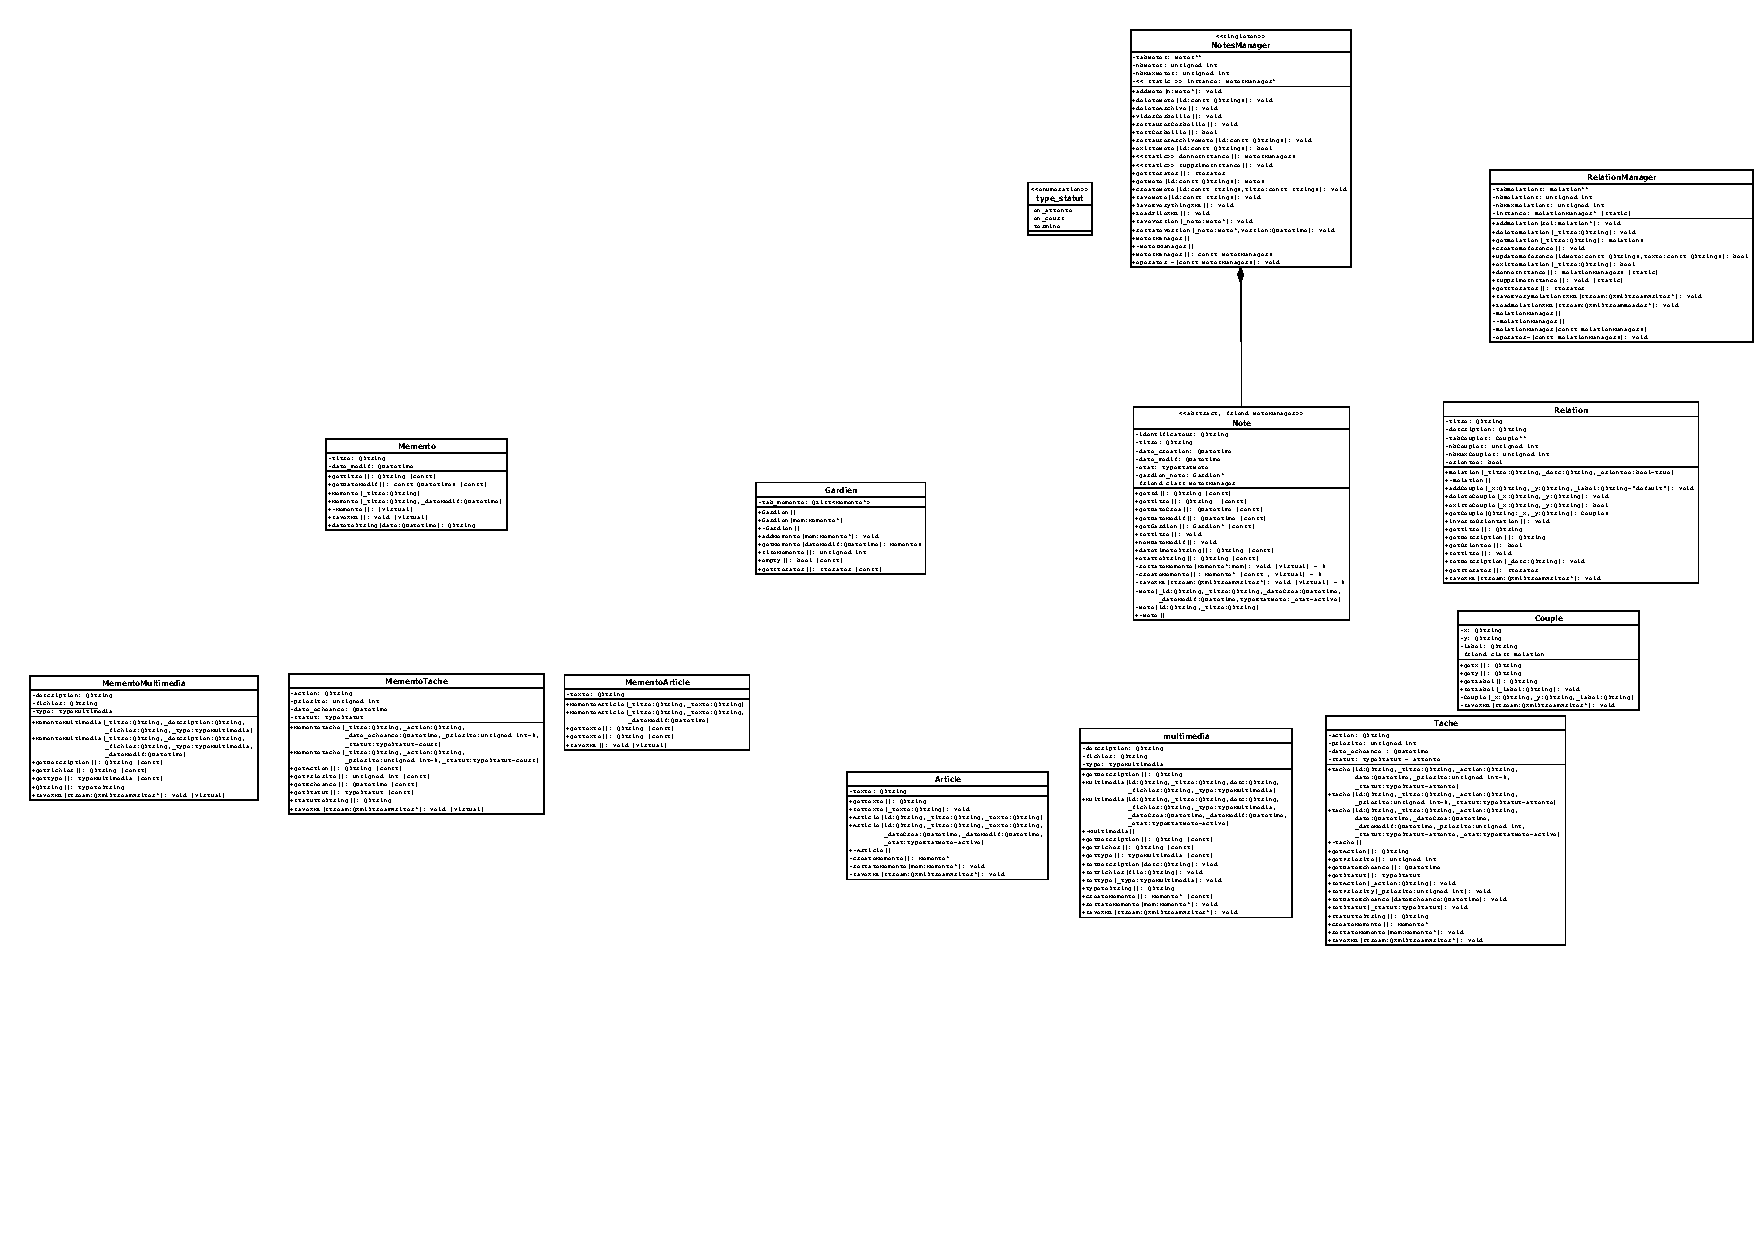
\includepdf[landscape=true]{UML.pdf}

\chapter{Choix de conception}

\section{Notes}

\subsection{Notes}

\subsection{NotesManager}

\section{Versionnage}

\section{Relations}

\subsection{Couples}

\subsection{Relations}

\subsection{RelationsManager}

\section{Sauvegarde et chargement des fichiers}

\section{Interface}

\section{Préférences}

\section{Édition}

\chapter{Conclusion}

\end{document}